%% SECTION HEADER /////////////////////////////////////////////////////////////////////////////////////
\section{Determination of the \acl{madif}}
\label{sec:determination}

%% SECTION CONTENT ////////////////////////////////////////////////////////////////////////////////////
The \ac{madif} was determined based on the function best fitted to indices selected in the previous subsection.
Since the numerically obtained indices took the shape of a non-linear function, several curves were assumed to find the best fit.
These functions were defined in the general form as follows
\begin{eqnarray}
	y_1(x,a_i) & = & \frac{a_1x}{x+a_2}+a_3,
	\label{eq:function_1}\\
	y_2(x,a_i) & = & a_1\sqrt{x} + a_2x+a_3,
	\label{eq:function_2}\\
	y_3(x,a_i) & = & \frac{a_1x}{\sqrt{a_2 + a_3x^2}}+a_4,\label{eq:function_3} 
\end{eqnarray}
where \(a_i\) are the coefficients of the functions.
The coefficients were determined by built-in function of Matlab named \verb+fminsearch+, which searches for the minimum of a problem specified by \(\min\limits_a f(x,a)\), and the function to be optimised was assumed to be \(f(x,a)=\left\|DI_{num} - y(x,a_i)\right\|\), where \(\left\|\cdot\right\|\) means Euclidean norm.
A criterion for evaluating the fit of the curve to simulation results was a mean absolute error defined as follows
\begin{eqnarray}
	\delta^{\mathrm{fit}} = \frac{1}{\mathrm{n^{DI}}}\sum_{i=1}^{\mathrm{n^{DI}}} \left|\frac{\mathrm{DI^i_{num}}-y(w_d^i)}{\mathrm{DI^i_{num}}}\right|\times100\%,
\end{eqnarray}
where \(\mathrm{n^{DI}}\) is the number of index points.
The examples of the results for \ac{rmsd} are presented in Table~\ref{tab:fit_RMSD_full_FCGM} based on the \ac{fcgm} and in Table~\ref{tab:fit_RMSD_full_HCGM} for the \ac{hcgm}.
The empty cells in the tables mean that the function was fitted with an error of more than 20\%.
The \ac{di} was no longer taken into account if the fit function was not established.
Although prepared, the presentation of a similar summary for the remaining cases was omitted for the Chapter's clarity.
Ultimately, the most fitted function was Eq.~(\ref{eq:function_1}) and Eq.~(\ref{eq:function_2}) for the most \acp{di}.
The best fitted functions were selected to determine the \ac{madif}.

\begin{table}[!tbh]
	\small
	\tabcolsep=0.1cm
	\centering
	\caption{\label{tab:fit_RMSD_full_FCGM} The errors of the functions fitted to the \acf{rmsd} based on full-length windowed signals and the \acf{fcgm}}
	\begin{tabular}{ccccccccccccccc}
		\toprule
		\multirow{3}{*}{\rotatebox[origin=c]{90}{Frequency}} & \multicolumn{7}{c}{\ac{fcgm} - core} & \multicolumn{7}{c}{\ac{fcgm} - interface}\\
		& \multirow{2}{*}{\rotatebox[origin=c]{90}{DI\(_{num}\)}} & \multicolumn{2}{c}{Eq.~(\ref{eq:function_1})} & \multicolumn{2}{c}{Eq.~(\ref{eq:function_2})} & \multicolumn{2}{c}{Eq.~(\ref{eq:function_3})} &
		\multirow{2}{*}{\rotatebox[origin=c]{90}{DI\(_{num}\)}} & \multicolumn{2}{c}{Eq.~(\ref{eq:function_1})} & \multicolumn{2}{c}{Eq.~(\ref{eq:function_2})} & \multicolumn{2}{c}{Eq.~(\ref{eq:function_3})}\\
		& & \(y(w_d^i)\)& \(\delta^{\mathrm{fit}}\) & \(y(w_d^i)\) & \(\delta^{\mathrm{fit}}\) & \(y(w_d^i)\) & \(\delta^{\mathrm{fit}}\) & & \(y(w_d^i)\)& \(\delta^{\mathrm{fit}}\) & \(y(w_d^i)\) & \(\delta^{\mathrm{fit}}\) & \(y(w_d^i)\) & \(\delta^{\mathrm{fit}}\)\\
		\midrule
		\multirow{7}{*}{\rotatebox[origin=c]{90}{100 \unit{\kHz}}} & 1.00 & 1.00 & \multirow{7}{*}{\rotatebox[origin=c]{90}{\textcolor{green}{1.50}}} & 1.00 & \multirow{7}{*}{\rotatebox[origin=c]{90}{1.70}} & 1.00 & \multirow{7}{*}{\rotatebox[origin=c]{90}{1.92}} & 1.00 & 1.00 & \multirow{7}{*}{\rotatebox[origin=c]{90}{\textcolor{green}{1.11}}} & 1.00 & \multirow{7}{*}{\rotatebox[origin=c]{90}{1.45}} & 1.00 & \multirow{7}{*}{\rotatebox[origin=c]{90}{1.31}} \\
		& 0.83 & 0.85 & & 0.88 & & 0.84 & & 0.92 & 0.92 & & 0.90 & & 0.94 & \\ 
		& 0.82 & 0.80 & & 0.82 & & 0.79 & & 0.85 & 0.84 & & 0.83 & & 0.85 & \\ 
		& 0.80 & 0.78 & & 0.79 & & 0.78 & & 0.79 & 0.79 & & 0.79 & & 0.80 & \\ 
		& 0.76 & 0.78 & & 0.78 & & 0.78 & & 0.76 & 0.77 & & 0.76 & & 0.77 & \\ 
		& 0.77 & 0.77 & & 0.77 & & 0.78 & & 0.73 & 0.75 & & 0.74 & & 0.76 & \\ 
		& 0.75 & 0.77 & & 0.78 & & 0.78 & & 0.75 & 0.73 & & 0.72 & & 0.75 & \\
		\midrule
		\multirow{7}{*}{\rotatebox[origin=c]{90}{150 \unit{\kHz}}} & 1.00 & 1.00 & \multirow{7}{*}{\rotatebox[origin=c]{90}{3.10}} & 1.00 & \multirow{7}{*}{\rotatebox[origin=c]{90}{\textcolor{green}{1.28}}} & 1.00 & \multirow{7}{*}{\rotatebox[origin=c]{90}{6.83}} & 1.00 & 1.00 & \multirow{7}{*}{\rotatebox[origin=c]{90}{1.32}} & 1.00 & \multirow{7}{*}{\rotatebox[origin=c]{90}{\textcolor{green}{0.73}}} & 1.00 & \multirow{7}{*}{\rotatebox[origin=c]{90}{4.85}} \\
		& 0.89 & 0.95 & & 0.92 & & 0.97 & & 0.93 & 0.96 & & 0.95 & & 0.97 & \\ 
		& 0.85 & 0.87 & & 0.85 & & 0.91 & & 0.89 & 0.89 & & 0.88 & & 0.92 & \\ 
		& 0.80 & 0.81 & & 0.79 & & 0.85 & & 0.83 & 0.83 & & 0.82 & & 0.87 & \\ 
		& 0.74 & 0.76 & & 0.74 & & 0.80 & & 0.76 & 0.77 & & 0.77 & & 0.82 & \\ 
		& 0.68 & 0.71 & & 0.70 & & 0.75 & & 0.71 & 0.72 & & 0.72 & & 0.76 & \\ 
		& 0.64 & 0.67 & & 0.65 & & 0.70 & & 0.67 & 0.68 & & 0.67 & & 0.71 & \\ 
		\bottomrule
	\end{tabular}
\end{table}

\begin{table}[!tbh]
	\small
	\tabcolsep=0.1cm
	\centering
	\caption{\label{tab:fit_RMSD_full_HCGM} The errors of the functions fitted to the \acf{rmsd} based on full-length windowed signals and the \acf{hcgm}}
	\begin{tabular}{ccccccccccccccc}
		\toprule
		\multirow{3}{*}{\rotatebox[origin=c]{90}{Frequency}} & \multicolumn{7}{c}{\ac{hcgm} - core} & \multicolumn{7}{c}{\ac{hcgm} - interface}\\
		& \multirow{2}{*}{\rotatebox[origin=c]{90}{DI\(_{num}\)}} & \multicolumn{2}{c}{Eq.~(\ref{eq:function_1})} & \multicolumn{2}{c}{Eq.~(\ref{eq:function_2})} & \multicolumn{2}{c}{Eq.~(\ref{eq:function_3})} &
		\multirow{2}{*}{\rotatebox[origin=c]{90}{DI\(_{num}\)}} & \multicolumn{2}{c}{Eq.~(\ref{eq:function_1})} & \multicolumn{2}{c}{Eq.~(\ref{eq:function_2})} & \multicolumn{2}{c}{Eq.~(\ref{eq:function_3})}\\
		& & \(y(w_d^i)\)& \(\delta^{\mathrm{fit}}\) & \(y(w_d^i)\) & \(\delta^{\mathrm{fit}}\) & \(y(w_d^i)\) & \(\delta^{\mathrm{fit}}\) & & \(y(w_d^i)\)& \(\delta^{\mathrm{fit}}\) & \(y(w_d^i)\) & \(\delta^{\mathrm{fit}}\) & \(y(w_d^i)\) & \(\delta^{\mathrm{fit}}\)\\
		\midrule
		\multirow{7}{*}{\rotatebox[origin=c]{90}{100 \unit{\kHz}}} & 1.00 & 1.00 & \multirow{7}{*}{\rotatebox[origin=c]{90}{\textcolor{green}{5.37}}} & 1.00 & \multirow{7}{*}{\rotatebox[origin=c]{90}{9.85}} & \multirow{7}{*}{-} & \multirow{7}{*}{-} & 1.00 & 1.00 & \multirow{7}{*}{\rotatebox[origin=c]{90}{7.40}} & 1.00 & \multirow{7}{*}{\rotatebox[origin=c]{90}{\textcolor{green}{6.22}}} & 1.00 & \multirow{7}{*}{\rotatebox[origin=c]{90}{11.15}} \\
		& 0.55 & 0.57 & & 0.71 & & & & 0.67 & 0.75 & & 0.74 & & 0.80 & \\ 
		& 0.57 & 0.53 & & 0.58 & & & & 0.61 & 0.57 & & 0.59 & & 0.58 & \\ 
		& 0.57 & 0.52 & & 0.54 & & & & 0.53 & 0.50 & & 0.51 & & 0.51 & \\ 
		& 0.48 & 0.51 & & 0.52 & & & & 0.45 & 0.46 & & 0.46 & & 0.48 & \\ 
		& 0.50 & 0.51 & & 0.53 & & & & 0.35 & 0.44 & & 0.42 & & 0.47 & \\ 
		& 0.47 & 0.51 & & 0.55 & & & & 0.42 & 0.42 & & 0.40 & & 0.46 & \\ 
		\midrule
		\multirow{7}{*}{\rotatebox[origin=c]{90}{150 \unit{\kHz}}} & 1.00 & 1.00 & \multirow{7}{*}{\rotatebox[origin=c]{90}{0.51}} & 1.00 & \multirow{7}{*}{\rotatebox[origin=c]{90}{\textcolor{green}{0.33}}} & 1.00 & \multirow{7}{*}{\rotatebox[origin=c]{90}{2.41}} & 1.00 & 1.00 & \multirow{7}{*}{\rotatebox[origin=c]{90}{\textcolor{green}{0.79}}} & 1.00 & \multirow{7}{*}{\rotatebox[origin=c]{90}{\textcolor{green}{0.79}}} & \multirow{7}{*}{-} & \multirow{7}{*}{-} \\
		& 0.96 & 0.97 & & 0.97 & & 0.98 & & 0.95 & 0.95 & & 0.94 & & & \\ 
		& 0.93 & 0.93 & & 0.93 & & 0.95 & & 0.88 & 0.89 & & 0.89 & & & \\ 
		& 0.89 & 0.89 & & 0.89 & & 0.91 & & 0.84 & 0.85 & & 0.85 & & & \\ 
		& 0.85 & 0.85 & & 0.85 & & 0.88 & & 0.82 & 0.82 & & 0.82 & & & \\ 
		& 0.81 & 0.81 & & 0.81 & & 0.84 & & 0.80 & 0.79 & & 0.79 & & & \\ 
		& 0.77 & 0.78 & & 0.78 & & 0.80 & & 0.76 & 0.77 & & 0.76 & & & \\ 
		\bottomrule
	\end{tabular}
\end{table}

Then all selected \acp{di} and their fitted functions were compared with experimental results.
The best results were obtained for the \ac{rmsd} and the \ac{cc} based on the full-length signals at 100 \unit{kHz}. 
Those indices are presented in Figures~\ref{fig:madif_rmsd_best} and \ref{fig:madif_cc_best}, respectively.
\begin{figure}[!tbh]
	\begin{center}
		\includegraphics[width=0.95\textwidth]{Chapter_7/MADIF_RMSD_100_best_err}
	\end{center}
	\caption{(\textbf{a}) Comparison of the \acl{madif} based on the \acf{rmsd} and the experimental results, and (\textbf{b}) the percentage error between them}
	\label{fig:madif_rmsd_best}
\end{figure}

\begin{figure}[!tbh]
	\begin{center}
		\includegraphics[width=0.95\textwidth]{Chapter_7/MADIF_CC_100_best_err}
	\end{center}
	\caption{(\textbf{a}) Comparison of the \acf{madif} based on \acf{cc} and the experimental results, and (\textbf{b}) the percentage error between them}
	\label{fig:madif_cc_best}
\end{figure}

Both indices achieved the lowest error around 5\% for the \ac{fcgm}, with the interface elements removed as the damage model.
The indices were also in very good agreement for the \ac{fcgm} with removed cells as a damage model.
In the case of the \ac{hcgm}, unsatisfactory results were obtained, as none of the indices correspond to the experimental ones with an error of less than 20\%.
What may be relevant here is that the wave continuously transmits energy to the core throughout its propagation.
In contrast, in the case of the \ac{fcgm}, the wave transmits energy incidentally, when it encounters the core walls.
\pagebreak

According to the analysis, the \ac{rmsd} and the \ac{cc} based on the \ac{fcgm} and full-length signals at 100 \unit{kHz} were chosen as the \ac{madif}.
From Eq. (\ref{eq:function_1}), they were defined as follows:
\begin{eqnarray}
	MADIF^{RMSD}(w_d) & = & {13.44w_d}/(w_d+38.12)+0.64,
	\label{eq:MADIF_RMSD}\\
	MADIF^{CC}(w_d) & = & 16.62w_d/(w_d+133.05)+0.88.
	\label{eq:MADIF_CC}
\end{eqnarray}

The comparison of the \ac{madif} and the \ac{edif} based on the \ac{rmsd} and the \ac{cc} are presented in Figure~\ref{fig:madif_20}.
The \ac{edif} was found based on experimental measurements, using the fit function from Eq.~(\ref{eq:function_1}) (the same as the \ac{madif}).
The \ac{rmsd} is in excellent agreement with the experimentally obtained index, achieving an absolute error of less than 4 mm over the full range of damage.
The result of the \ac{cc} is less satisfactory, but it also agrees with the experimentally obtained index.
The absolute error is less than 9 mm.
\pagebreak
Both indices can be used to estimate the damage size in the assumed scenario with a proposed approximation function.
\begin{figure}[!tbh]
	\begin{center}
		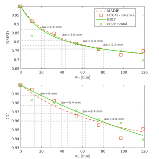
\includegraphics[width=1.0\textwidth]{Chapter_7/MADIF_20}
	\end{center}
	\caption{The \acl{madif} and the \acf{edif} based on the \acf{rmsd} 100 \unit{\kHz}}
	\label{fig:madif_20}
\end{figure}
